% ============================================================
%  PRISM — NeurIPS 2026 Anonymous Submission
%  Architecture details verified against codebase (2026-03).
% ============================================================
\documentclass{article}

% ── NeurIPS 2026 style (anonymous double-blind submission) ──
\usepackage{neurips_2026}

\usepackage[utf8]{inputenc}
\usepackage[T1]{fontenc}
\usepackage{hyperref}
\usepackage{url}
\usepackage{booktabs}
\usepackage{amsmath}
\usepackage{amssymb}
\usepackage{amsfonts}
\usepackage{graphicx}
\usepackage{xcolor}
\usepackage{microtype}
\usepackage{nicefrac}
\usepackage{multirow}
\usepackage{subcaption}
\usepackage{enumitem}
\usepackage{colortbl}   % \rowcolor

% ── PRISM brand color ────────────────────────────────────────
\definecolor{prismblue}{RGB}{29, 78, 216}

% ── Custom macros ───────────────────────────────────────────
\newcommand{\Rbb}{\mathbb{R}}
\newcommand{\todo}[1]{\textcolor{red}{[\textbf{TODO:} #1]}}
\newcommand{\answerYes}[0]{\textcolor{green}{\textbf{Yes}}}
\newcommand{\answerNo}[0]{\textcolor{red}{\textbf{No}}}
\newcommand{\answerNA}[0]{\textcolor{gray}{\textbf{N/A}}}
\newcommand{\answerTODO}[0]{\textcolor{orange}{\textbf{TODO}}}
\newcommand{\justificationTODO}{\textcolor{orange}{\textit{TODO}}}

% ── Title ───────────────────────────────────────────────────
\title{\textcolor{prismblue}{\textbf{PRISM}}: Human \textcolor{prismblue}{P}oint Cloud \textcolor{prismblue}{R}econstruction v\textcolor{prismblue}{i}a \\
       \textcolor{prismblue}{S}keleton-Guided Diffusion from \textcolor{prismblue}{M}mWave Radar}

\author{Anonymous Authors}

% ============================================================
\begin{document}
\maketitle

% ────────────────────────────────────────────────────────────
\begin{abstract}
mmWave radar enables all-weather, non-contact human sensing, yet its inherent
sparsity of 50--150 reflections per frame severely limits downstream body analysis.
Existing point cloud completion methods target dense rigid-object inputs and
fundamentally fail under the combination of extreme sparsity and non-rigid
topological variability of human bodies.
We present \textbf{PRISM}, a conditional latent diffusion framework for human
point cloud reconstruction from sparse mmWave radar.
SkelKD aligns noisy depth-camera skeletons to the radar coordinate frame via
cross-modal attention; HierVAE then encodes the sparse input into compact
$8\!\times\!120$ latent tokens through a six-level hierarchical VAE.
GeoAE simultaneously extracts a stable 128-point coarse geometric proxy from
the raw mmWave cloud; together with skeleton topology via a graph convolutional
network and action class label, this assembles a 145-token conditioning sequence
that guides a Dynamic Transformer to denoise the latent representation under
a VP-SDE framework.
On MM-Fi, PRISM significantly outperforms point cloud completion and generative
baselines on MMD-CD, COV-CD, and 1-NN-CD metrics while producing temporally
consistent, action-specific human point cloud sequences.
We further contribute OccluRadar-Human, the first dataset providing paired
complete and occluded mmWave captures with frame-level 3-D skeleton ground truth.
\end{abstract}

% ────────────────────────────────────────────────────────────
\section{Introduction}
\label{sec:intro}

mmWave radar has attracted growing interest for human body sensing due to its
ability to penetrate non-metallic obstacles, operate under complete darkness, and
preserve subject privacy~\cite{yang2023mmfi}.
Unlike LiDAR which yields thousands of points per frame, a mmWave radar typically
captures only 50--150 reflections from a human body, producing point clouds that
are simultaneously \emph{extremely sparse} and \emph{structurally incomplete}.
This sparsity bottleneck degrades downstream tasks such as human pose
estimation (HPE) and action recognition (HAR).

Recovering a complete human shape from such sparse observations is a
highly under-constrained problem demanding strong structural priors.
Point cloud completion methods---PCN~\cite{pcn}, PoinTr~\cite{pointr},
SnowflakeNet~\cite{snowflake}, LAKe-Net~\cite{lakenet}---are designed for
dense inputs ($>$2048 pts) from geometrically rigid objects (chairs, cars,
airplanes) in ShapeNet/PCN benchmarks, and fundamentally cannot handle the
combination of extreme sparsity ($<$256 pts) and high topological variability
of non-rigid human bodies.
Generative approaches such as LION~\cite{lion} and TIGER~\cite{tiger} operate
unconditionally or with weak semantic cues, lacking the skeleton-level structural
prior needed for occluded and view-dependent mmWave captures.

Our core observation is that the \emph{human skeleton} is a natural semantic
prior: 17 keypoints define the topological structure and joint-space constraints
of the body, serving as the bridge between sparse observation and complete human
shape.
In practice, depth cameras or IMUs provide coarse skeleton estimates; however,
calibration errors, occlusion, and coordinate-frame misalignments prevent raw
skeletons from being used directly as reliable geometric priors.

We present \textbf{PRISM}, an end-to-end framework for human point cloud
completion driven by skeleton guidance in a latent diffusion space.
Our main contributions are:
\begin{itemize}[leftmargin=1.5em,itemsep=1pt]
  \item \textbf{SkelKD} (Skeleton Keypoint Detector): a cross-modal attention
        module that regresses refined 3-D keypoints from sparse radar returns via
        learnable joint-query soft aggregation, eliminating coordinate-frame bias
        in depth-camera skeletons without any explicit calibration target.
  \item \textbf{HierVAE} (Hierarchical Point-Cloud VAE): a six-level hierarchical
        VAE that encodes variable-length sparse point clouds into a fixed-size
        structured latent space ($8\!\times\!120$ tokens), enabling stable diffusion
        at fixed resolution independent of input point count.
  \item \textbf{Condition Network:} unlike prior work using a single
        global condition vector, we inject (i)~skeleton topology via a 2-layer
        GCN over H36M-17 joints (17 tokens), (ii)~geometric coarse points from
        GeoAE (128 tokens), and (iii)~action class label, forming a
        145-token K/V sequence injected into every denoising layer of the
        Dynamic Transformer.
  \item \textbf{OccluRadar-Human:} the first paired dataset with
        complete/occluded mmWave captures and synchronized 3-D skeleton ground
        truth, validating PRISM in realistic through-obstacle sensing.
\end{itemize}

% ── Teaser figure ───────────────────────────────────────────
\begin{figure}[t]
  \centering
  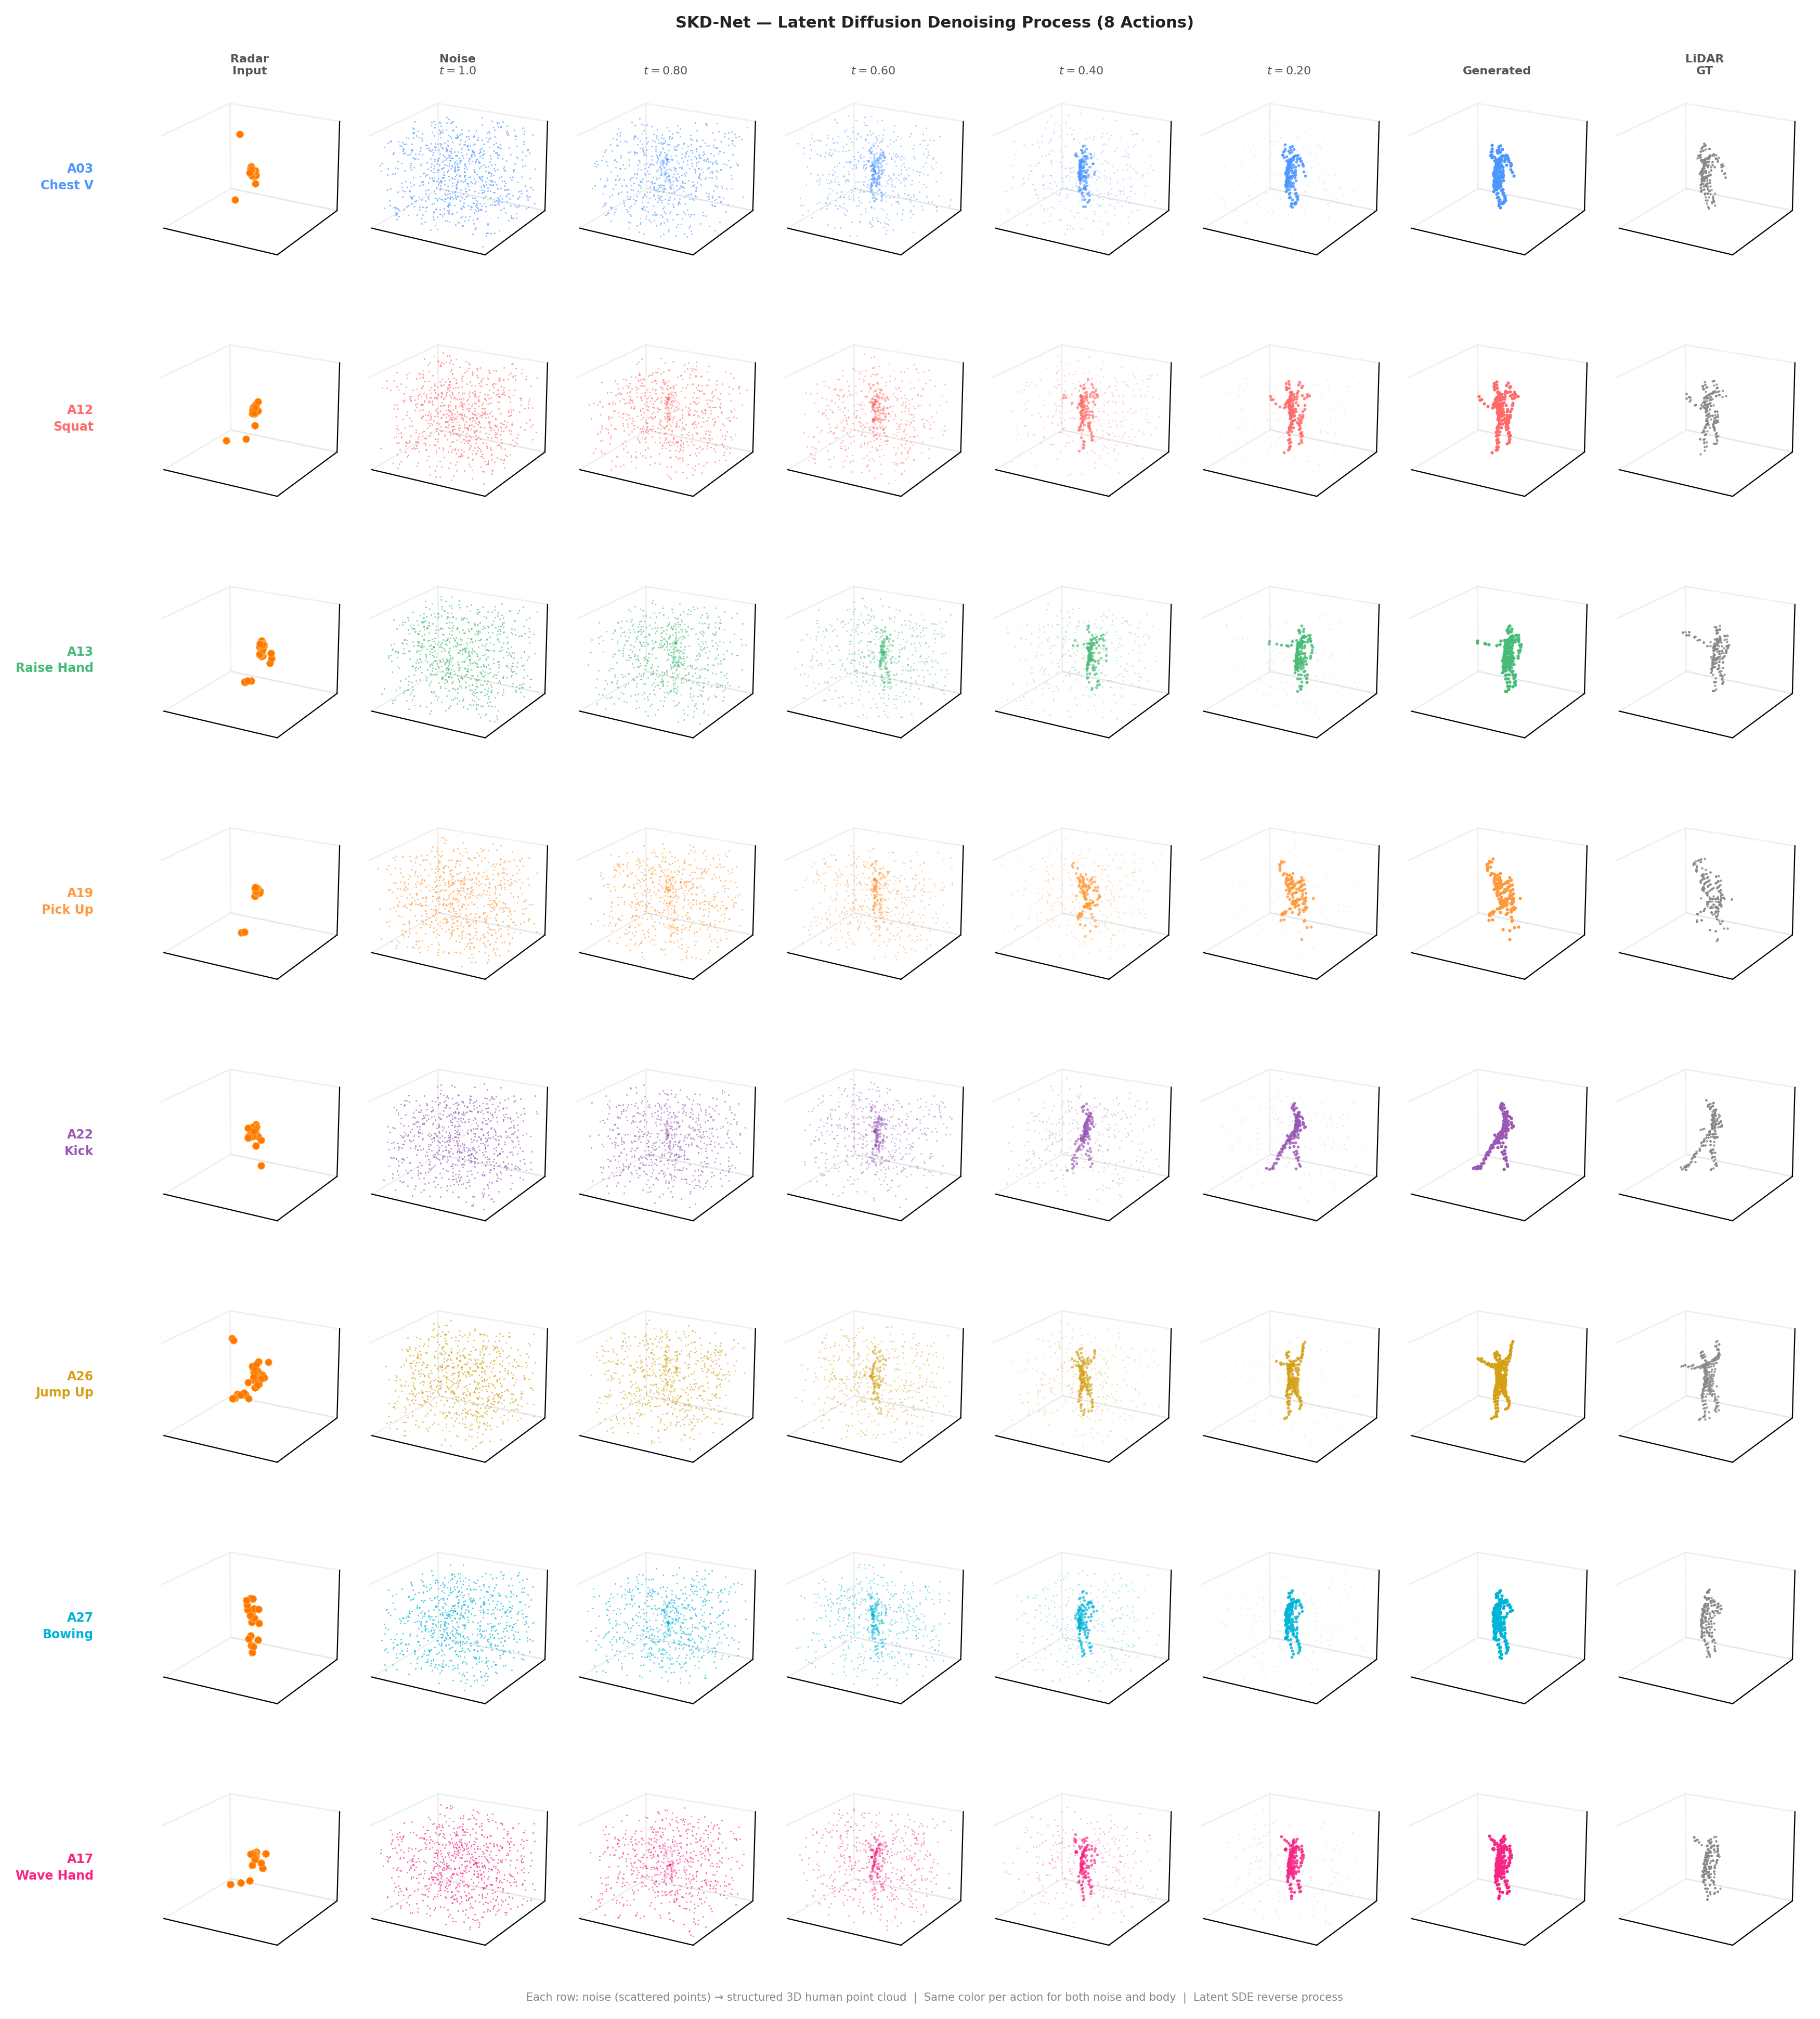
\includegraphics[width=\linewidth]{assets/diffusion_grid.png}
  \caption{
    \textbf{PRISM completion results on MM-Fi.}
    Each row shows one representative action.
    \textbf{Left to right:} sparse mmWave radar input (50--150 pts),
    SkelKD-refined skeleton,
    PRISM generated point cloud,
    LiDAR ground truth (256 pts).
    PRISM recovers topologically correct and naturally shaped human point
    clouds from extreme radar sparsity, guided solely by the sparse radar
    observation and a skeleton prior.
  }
  \label{fig:teaser}
\end{figure}

% ────────────────────────────────────────────────────────────
\section{Related Work}
\label{sec:related}

\paragraph{Point cloud completion.}
PCN~\cite{pcn} pioneered coarse-to-fine hierarchical decoding with FoldingNet
for global-feature-based generation.
PoinTr~\cite{pointr} reformulates completion as a set-to-set Transformer task
with geometry-aware proxy point grouping.
SnowflakeNet~\cite{snowflake} proposes skip-Transformer multi-scale upsampling.
LAKe-Net~\cite{lakenet} introduces unsupervised keypoint localization and surface
skeleton generation to model topology---most closely related to our approach.
However, all assume dense inputs ($>$2048 pts) and rigid object categories,
making them fundamentally unsuitable for mmWave human body completion.

\paragraph{Diffusion models for 3-D generation.}
LION~\cite{lion} proposes hierarchical VAE + DDM for unconditional point cloud
generation in shape latent space.
LDT~\cite{ldt} (our diffusion backbone) encodes point clouds into latent tokens
and uses a Dynamic Transformer for conditional denoising generation.
TIGER~\cite{tiger} introduces time-varying denoising for temporally consistent
generation.
Our work extends LDT by upgrading skeleton conditioning from a single global
vector to a joint GCN + coarse-geometry dual-path 145-token sequence-level
condition, and replacing FPS-based geometry aggregation with GeoAE.

\paragraph{mmWave human sensing.}
MM-Fi~\cite{yang2023mmfi} is the first large-scale multi-modal human sensing
dataset with precisely synchronized mmWave point clouds and 3-D skeleton
annotations.
mmPoint~\cite{mmpoint} processes mmWave point clouds directly for body sensing
but lacks a generative prior for distribution-faithful completion.
mmBody~\cite{mmbody} and RadarHD~\cite{radarhd} explore mmWave densification
but focus only on visible-region densification rather than semantic full-body
completion.
To our knowledge, PRISM is the first systematic study of complete human body
reconstruction from extremely sparse mmWave point clouds.

% ────────────────────────────────────────────────────────────
\section{Method}
\label{sec:method}

\subsection{Overview}

% ── Full architecture figure ─────────────────────────────────
\begin{figure}[t]
  \centering
  % ── 制图说明（供 Inkscape/PPT 制图参考）──────────────────
  % 左侧路径①（Condition Path）：
  %   [mmWave PC (B,N,3)]
  %     ├──→ [GeoAE]  →  coarse C (B,128,3)
  %     │                              ↓
  %     │         [Condition Net]  ←──────────────────────────┐
  %     │           GCN(17 tok)                               │
  %     │         + CoarseEnc(128 tok)  →  KV (B,256,145)    │
  %     │         + LabelEmb                                  │
  %     │                                                     │
  %     └──→ [SkelKD] ← [Depth Skel (B,17,3)]                │
  %              ↓ P̂(B,17,3)                                 │
  %         [HierVAE Enc]  →  Z₀ (B,8,120)                   │
  %                                   ↓                       │
  % 右侧路径②（Diffusion Path）：            Forward SDE       │
  %                                   ↓                       │
  %                               Z_t (noisy)                 │
  %                                   ↓  ←── KV (145 tok) ───┘
  %             [Dynamic Transformer (6 blocks, hidden=256)]
  %                     ←── t_emb + label_emb + g_s (AdaLN)
  %                                   ↓
  %                               Ẑ₀ (denoised)
  %                                   ↓
  %                        [HierVAE Dec]
  %                                   ↓
  %                           X_f (B,256,3)
  % ─────────────────────────────────────────────────────────
  \fbox{\parbox[c][7.2cm][c]{0.96\linewidth}{%
    \centering\small\color{gray}
    \textbf{[Fig.~2 — Full Architecture Diagram (placeholder)]}\\[6pt]
    \textbf{Path \textcircled{1}:}
    mmWave $\xrightarrow{\text{GeoAE}}$ Coarse $C$ (128 pts)
    $+$ Depth Skel $\xrightarrow{\text{SkelKD}}$ $\hat{P}$ (17 joints)\\
    $\hat{P} \xrightarrow{\text{HierVAE Enc}}$ $Z_0 \in\Rbb^{B\times8\times120}$
    \quad
    $[\hat{P},\,C] \xrightarrow{\text{Condition Network}}$
    $\mathrm{KV}\in\Rbb^{B\times256\times145}$\\[6pt]
    \textbf{Path \textcircled{2}:}
    $Z_0 \xrightarrow{\text{VP-SDE fwd}}Z_t
    \xrightarrow{\text{DynTransformer}(6\text{ blocks}),\;\mathrm{KV},\;t,\;y}
    \hat{Z}_0
    \xrightarrow{\text{HierVAE Dec}}X_f\!\in\!\Rbb^{B\times256\times3}$
  }}
  \caption{
    \textbf{PRISM architecture overview.}
    Path~\textcircled{1} (left) builds the three-stream condition signal and
    encodes the sparse point cloud into a clean latent $Z_0$.
    Path~\textcircled{2} (right) runs VP-SDE forward diffusion on $Z_0$,
    then a Dynamic Transformer denoises $Z_t$ conditioned on the 145-token K/V
    sequence, yielding $\hat{Z}_0$ decoded by the HierVAE into the final
    point cloud $X_f$.
  }
  \label{fig:arch}
\end{figure}

Figure~\ref{fig:arch} illustrates the two-path structure of PRISM.
\textbf{Path~\textcircled{1}} (condition path) takes sparse mmWave point cloud
$X\!\in\!\Rbb^{B\times N\times3}$ and raw depth-camera skeleton
$P_\text{raw}\!\in\!\Rbb^{B\times17\times3}$ as input.
SkelKD refines $P_\text{raw}$ to the radar coordinate frame, yielding
$\hat{P}\!\in\!\Rbb^{B\times17\times3}$.
GeoAE produces a 128-point geometric coarse proxy
$C\!\in\!\Rbb^{B\times128\times3}$ from the same mmWave input.
The HierVAE encodes the sparse point cloud into the clean latent
$Z_0\!\in\!\Rbb^{B\times8\times120}$.
The Condition Network assembles a 145-token K/V sequence from $\hat{P}$ and $C$.
\textbf{Path~\textcircled{2}} (diffusion path) corrupts $Z_0$ to $Z_t$ via a
VP-SDE, then a Dynamic Transformer (6 blocks) iteratively denoises under the
145-token condition and global signal $c$, yielding $\hat{Z}_0$ which the
HierVAE decoder maps to $X_f\!\in\!\Rbb^{B\times256\times3}$.

\subsection{Multimodal Coordinate Alignment}
\label{sec:align}

MM-Fi records three modalities with independent coordinate conventions.

\textbf{LiDAR} follows $(x_\text{depth}, y_\text{lateral}, z_\text{height})$.
Each frame is mean-centered and normalized to the unit sphere:
$\tilde{P}_L = (P_L - \bar{P}_L) / \max_i \|p_i - \bar{P}_L\|_2$.
Parameters $(\bar{P}_L, s_L)$ are retained for skeleton alignment.

\textbf{Skeleton.}
Depth-camera joints use axis order $(\text{lateral}, \text{height}, \text{depth})$.
We permute $P_S^{\text{aligned}} = P_S[:,\,[2,0,1]]$ and apply the LiDAR
normalization: $\tilde{P}_S = (P_S^{\text{aligned}} - \bar{P}_L) / s_L$.

\textbf{mmWave} point clouds are human-centered with a $\sim$3\,m systematic
offset from the LiDAR frame.
We independently normalize $\tilde{P}_M = (P_M^{\text{valid}} - \bar{P}_M)/s_M$,
filtering invalid points ($|p|>20$\,m or non-finite).
The residual coordinate offset is further corrected by SkelKD
(Section~\ref{sec:skelkd}).

\subsection{SkelKD: Skeleton Keypoint Detector}
\label{sec:skelkd}

\begin{figure}[t]
  \centering
  \fbox{\parbox[c][5.2cm][c]{0.92\linewidth}{%
    \centering\small\color{gray}
    \textbf{[Fig.~3 — SkelKD Architecture (placeholder)]}\\[6pt]
    mmWave $(B,N,3)$
    $\xrightarrow{\text{Conv1d}\;3\to64\to128\;\text{+BN}}$
    $f_\text{local}$ $(B,N,128)$
    $\xrightarrow{\text{MaxPool+MLP}\;128\to256}$
    $f_\text{global}$ $(B,256)$\\[4pt]
    Joint Embed $(17\times128)$ as $Q$;\ $f_\text{local}$ as $K,V$
    $\;\xrightarrow{\text{Cross-Attn}}\;$
    $f_\text{joint}$ $(B,17,128)$\\[4pt]
    $\mathrm{cat}[f_\text{joint},\,f_\text{global}^{\!\exp}]$ $(B,17,384)$
    $\xrightarrow{\text{Res-MLP}\;384\to256\to128\to3\;(\text{zero-init})}$
    $\Delta P$ $(B,17,3)$\\[4pt]
    $\hat{P} = P_\text{raw}+\Delta P$,\quad
    $\mathcal{L}=\mathcal{L}_\text{MPJPE}+0.1\,\mathcal{L}_\text{bone}$
  }}
  \caption{
    \textbf{SkelKD.}
    Learnable joint embeddings serve as Cross-Attention queries;
    sparse radar point features serve as keys and values.
    A zero-initialized residual MLP regresses per-joint 3-D corrections,
    ensuring near-identity initialization and stable early-training gradients.
  }
  \label{fig:skelkd}
\end{figure}

SkelKD (Skeleton Keypoint Detector) regresses a radar-space-aligned refined
skeleton $\hat{P}\!\in\!\Rbb^{B\times17\times3}$ from sparse mmWave $X$ and
the raw depth-camera skeleton $P_\text{raw}$, removing coordinate-frame bias
and occlusion-induced joint drift without any explicit calibration target.

\paragraph{PCN encoder.}
Two 1D-convolution layers ($3\!\to\!64\!\to\!128$, BatchNorm) produce per-point
local features $f_\text{local}\!\in\!\Rbb^{B\times N\times128}$.
Symmetric max-pooling followed by a 2-layer MLP ($128\!\to\!256$) yields the
global context vector $f_\text{global}\!\in\!\Rbb^{B\times256}$.

\paragraph{Joint feature aggregator.}
Under extreme sparsity ($N\!<\!128$), nearest-neighbor joint-to-point mapping
degenerates for occluded joints.
A learnable $17\!\times\!128$ joint embedding table serves as Cross-Attention
query $Q$, with $f_\text{local}$ as keys $K$ and values $V$:
\begin{equation}
  f_\text{joint} = \mathrm{softmax}\!\left(\tfrac{QK^\top}{\sqrt{d}}\right)V,
  \quad Q\!\in\!\Rbb^{17\times128},\ K,V\!\in\!\Rbb^{N\times128}.
\end{equation}
When a joint is occluded, attention weights spread uniformly over all $N$ points
rather than collapsing to zero, and the injected global feature compensates.

\paragraph{Residual regression head.}
Concatenated features $(B,17,384)$ pass through a shared-weight residual MLP
($384\!\to\!256\!\to\!128\!\to\!3$, zero-initialized output layer):
\begin{equation}
  \hat{P} = P_\text{raw}
            + \mathrm{MLP}_\text{res}\!\left([f_\text{joint}\,\|\,f_\text{global}]\right),
  \quad \hat{P}\!\in\!\Rbb^{B\times17\times3}.
\end{equation}
Training loss:
$\mathcal{L}_\text{SkelKD} = \mathcal{L}_\text{MPJPE} + 0.1\,\mathcal{L}_\text{bone}$,
with Gaussian noise augmentation ($\sigma\!=\!0.03$) and random joint occlusion
(30\% probability, $\leq\!4$ joints zeroed).
SkelKD weights are frozen after pre-training.

\subsection{HierVAE: Hierarchical Point-Cloud VAE}
\label{sec:compressor}

HierVAE (Hierarchical Point-Cloud VAE) encodes a variable-length sparse point
cloud into a fixed-size structured latent $Z_0\!\in\!\Rbb^{B\times8\times120}$
and decodes latent tokens back to a dense point cloud.

\paragraph{Hierarchical encoder.}
Six hierarchical levels each apply a local grouper ($k\!=\!32$ neighbors,
radius-based), a ResidualBlock with multi-head self-attention
($d\!=\!128$, 4~heads), and MLP expansion.
Each level produces per-level VAE statistics
$(\mu_l,\log\sigma_l)\!\in\!\Rbb^{B\times z_\text{scale}\times2z_\text{dim}}$
($z_\text{scale}\!=\!8$, $z_\text{dim}\!=\!20$).
Concatenating all six levels along the feature dimension yields
$Z_0\!\in\!\Rbb^{B\times8\times120}$ ($6\!\times\!20\!=\!120$).
ActNorm layers ensure numerically stable VAE training.

\paragraph{Decoder.}
A learnable initial set (prior $\mu_0, \log\sigma_0$) serves as seed points,
iteratively updated via posterior estimation conditioned on each latent level
through DecoderBlocks.
The output count $K\!=\!256$ is decoupled from the encoder and can be adjusted
at inference without retraining.

\paragraph{Training objective.}
$\mathcal{L}_\text{HierVAE}
  = \mathcal{L}_\text{CD} + \mathcal{L}_\text{EMD}
  + \lambda_\text{KL}\,\mathcal{L}_\text{KL}$,\;
$\lambda_\text{KL}\!=\!10^{-4}$.

\subsection{GeoAE: Geometric Auto-Encoder}
\label{sec:aae}

\begin{figure}[t]
  \centering
  \fbox{\parbox[c][5.0cm][c]{0.92\linewidth}{%
    \centering\small\color{gray}
    \textbf{[Fig.~4 — GeoAE + Condition Network (placeholder)]}\\[5pt]
    \textbf{GeoAE:}\quad
    mmWave $(B,N,3)$
    $\xrightarrow{\text{PCN-Enc}\;3\to128\to256}$ $f_g(B,256)$
    $\xrightarrow{\text{SeedGen (ConvT + MLP-Res}\times3)}$ $C(B,128,3)$\\[5pt]
    \textbf{Condition Network:}\\
    $\hat{P}(B,17,3)\xrightarrow{\text{GCN-2L (H36M-17)}\;3\to128\to256}
      F_s(B,17,256)\xrightarrow{\mathrm{Proj}}\mathrm{KV}_s(B,256,17)$\\
    $C(B,128,3)\xrightarrow{\text{Conv1d}\;3\to256\to256}
      \mathrm{KV}_c(B,256,128)$\\
    $\mathrm{KV}=\mathrm{cat}[\mathrm{KV}_s,\,\mathrm{KV}_c]
      \in\Rbb^{B\times256\times145}$\\
    $g_s=\mathrm{MeanPool}(F_s)\Rightarrow
      c = t_\mathrm{emb}+y_\mathrm{emb}+\mathrm{Linear}(g_s)$
      \;(AdaLayerNorm modulation)
  }}
  \caption{
    \textbf{GeoAE (top) and Condition Network (bottom).}
    GeoAE distills raw mmWave into 128 stable coarse points.
    The Condition Network concatenates 17 skeleton GCN tokens and 128 coarse
    geometry tokens into a 145-token K/V sequence.
    A global signal $c$ dynamically modulates every AdaLayerNorm in the
    Dynamic Transformer.
  }
  \label{fig:condnet}
\end{figure}

GeoAE (Geometric Auto-Encoder) converts the raw mmWave point cloud into 128
canonical coarse points $C\!\in\!\Rbb^{B\times128\times3}$ that serve as a
stable geometric proxy for Condition Network, even under heavy occlusion.
It is jointly trained with the diffusion stage.

\paragraph{Encoder.}
Two Conv1d layers ($3\!\to\!128\!\to\!256$) extract per-point features;
symmetric max-pooling yields global feature $f_g\!\in\!\Rbb^{B\times256}$.

\paragraph{Seed generator (decoder).}
A transposed convolution unfolds $f_g$ into 128 seed points,
followed by three MLP-Residual blocks and a final Conv1d
($128\!\to\!64\!\to\!3$).

\paragraph{Training objective.}
$\mathcal{L}_\text{AE} = 0.1\,\mathcal{L}_\text{CD}(C, X_\text{GT})$,
optimized jointly with the diffusion score-matching loss.

\subsection{Condition Network}
\label{sec:condnet}

The Condition Network assembles the three-stream condition signal injected into
every denoising layer of the Dynamic Transformer (Fig.~\ref{fig:condnet}).

\paragraph{Stream \textcircled{1}: Skeleton GCN encoder.}
The refined skeleton $\hat{P}$ is encoded by a 2-layer GCN defined on the
H36M-17 topology (Pelvis--Spine--Thorax--Head trunk;
bilateral hip--knee--ankle legs; bilateral shoulder--elbow--wrist arms).
The symmetrically normalized adjacency matrix
$\hat{A} = D^{-1/2}(A+I)D^{-1/2}$ drives the GCN update:
\begin{equation}
  H^{(l+1)} = \sigma\!\left(\hat{A}\,H^{(l)}\,W^{(l)}\right),
\end{equation}
with GELU activation and LayerNorm.
The 2-layer GCN maps $17\!\times\!3\!\to\!17\!\times\!256$, producing node
features $F_s$ projected to $\mathrm{KV}_s\!\in\!\Rbb^{B\times256\times17}$.
The global pool $g_s\!=\!\mathrm{MeanPool}(F_s)$ feeds into $c$.

\paragraph{Stream \textcircled{2}: Coarse geometry encoder.}
GeoAE's 128 coarse points $C$ are encoded by two Conv1d layers
($3\!\to\!256\!\to\!256$) to yield
$\mathrm{KV}_c\!\in\!\Rbb^{B\times256\times128}$.
Unlike FPS-based aggregation (which degenerates at $N\!\sim\!50$),
GeoAE provides stable and complete geometry even under heavy occlusion.

\paragraph{K/V token concatenation.}
\begin{equation}
  \mathrm{KV}
    = \mathrm{cat}[\mathrm{KV}_s,\,\mathrm{KV}_c]
    \;\in\;\Rbb^{B\times256\times145},
\end{equation}
forming a 145-token K/V sequence injected into every Cross-Attention layer of
the Dynamic Transformer.

\paragraph{Stream \textcircled{3}: Action class label.}
Action label $y\!\in\!\{0,\ldots,7\}$ is embedded as
$e_y\!=\!\mathrm{LabelEmb}(y)$.
The joint global modulation signal is:
\begin{equation}
  c = e_t + e_y + \mathrm{Linear}(g_s),
\end{equation}
where $e_t$ is the diffusion time embedding.
$c$ modulates scale/shift in every Adaptive LayerNorm of the Dynamic Transformer.
During training, each stream is independently dropped with 10\% probability for
Classifier-Free Guidance (CFG).

\subsection{Forward Diffusion and Dynamic Transformer}
\label{sec:diffusion}

\paragraph{VP-SDE forward process.}
Starting from the clean latent $Z_0$ from the HierVAE encoder, a
variance-preserving SDE adds Gaussian noise over $T\!=\!1000$ steps:
\begin{equation}
  q(Z_t\mid Z_{t-1})
    = \mathcal{N}\!\left(Z_t;\,\sqrt{1-\beta_t}\,Z_{t-1},\,\beta_t I\right),
\end{equation}
with linear noise schedule $\beta_1\!=\!0.1$ to $\beta_T\!=\!20$.
Diffusion operates entirely in the $8\!\times\!120$ latent space.

\paragraph{Dynamic Transformer denoising network.}
The Dynamic Transformer consists of 6 denoising blocks (hidden dim 256,
4~attention heads).
Each block: (1)~project $Z_t$ and fuse with $e_t$ to form Query;
(2)~inject the 145-token $\mathrm{KV}$ as Cross-Attention keys/values;
(3)~feed through residual connection into Adaptive LayerNorm modulated by $c$;
(4)~apply element-wise feed-forward.
At inference, the ancestral sampler with 200 steps is used for efficiency.

\subsection{Progressive Four-Stage Training}
\label{sec:training}

\textbf{Stage~1 (SkelKD).}
Train SkelKD with MPJPE + bone loss; noise + joint-occlusion augmentation.
Freeze after convergence.

\textbf{Stage~2 (HierVAE).}
Train encoder and decoder with $\mathcal{L}_\text{CD}+\mathcal{L}_\text{EMD}
+10^{-4}\mathcal{L}_\text{KL}$.

\textbf{Stage~3 (LDT).}
Freeze HierVAE.
Jointly train Dynamic Transformer, Condition Network, GeoAE, and CFG.
Objective: score-matching loss (L2) + coarse auxiliary CD ($\lambda\!=\!0.1$).

\textbf{Stage~4 (Joint fine-tuning).}
Unfreeze all except SkelKD; optimize end-to-end.

% ────────────────────────────────────────────────────────────
\section{Dataset}
\label{sec:dataset}

\subsection{MM-Fi}
\label{sec:mmfi}

MM-Fi~\cite{yang2023mmfi} comprises RGB, depth, LiDAR, mmWave, and WiFi-CSI
across 40 subjects, 4 environments, and 27 action classes ($>$320k frames).
Our protocol:
\begin{itemize}[leftmargin=1.5em,itemsep=1pt]
  \item \textbf{Actions:} 8 classes --- A03 (chest-V), A12 (squat), A13
        (raise-hand-L), A17 (wave-hand-L), A19 (pick-up), A22 (kick-L),
        A26 (jump-up), A27 (bowing).
  \item \textbf{Subjects:} Train S01--S07; Validation S08--S10; Env.\ E01.
  \item \textbf{Input:} mmWave sparse PC ($N\!\leq\!256$ pts, actual 50--150);
        H36M-17 skeleton from depth camera (aligned to LiDAR frame).
  \item \textbf{GT:} LiDAR point cloud subsampled to 256 pts per frame.
\end{itemize}

\subsection{OccluRadar-Human}
\label{sec:occludata}

\begin{figure}[t]
  \centering
  \fbox{\parbox[c][4.8cm][c]{0.90\linewidth}{%
    \centering\small\color{gray}
    \textbf{[Fig.~5 --- OccluRadar-Human (placeholder)]}\\[6pt]
    \textbf{Left:} Sensor layout ---
    2$\times$ TI IWR6843 (clear-view + occluded) + Intel RealSense D435i\\
    Clear radar: complete human PC (GT); Occluded radar: 18\,mm wooden barrier\\[5pt]
    \textbf{Right:} Sample paired point clouds at three occlusion levels\\
    Row 1: No occlusion \quad Row 2: Partial \quad Row 3: Heavy
  }}
  \caption{
    \textbf{OccluRadar-Human.}
    Left: dual-radar + depth-camera collection setup.
    Right: paired mmWave point cloud samples across occlusion levels.
    One TI IWR6843 records a complete human body as GT; the other captures
    attenuated returns from behind an 18\,mm wooden panel simulating
    through-wall/obstacle scenarios.
  }
  \label{fig:occludata}
\end{figure}

Existing public mmWave datasets are collected in obstacle-free environments.
OccluRadar-Human provides paired complete/occluded captures for through-obstacle
evaluation.
Two TI IWR6843 radars (clear-view + occluded) and one Intel RealSense D435i
depth camera synchronously capture the same subject; sensors are extrinsic-calibrated
to a shared world coordinate.
We collected \todo{N} subjects performing \todo{M} action classes
($\sim$297 frames/sequence).
To our knowledge, OccluRadar-Human is the first dataset providing paired
complete/occluded mmWave point clouds with frame-level 3-D skeleton ground truth.

% ────────────────────────────────────────────────────────────
\section{Experiments}
\label{sec:exp}

\subsection{Implementation Details}
\label{sec:impl}

\textbf{Architecture.}
SkelKD: local feat 128, global feat 256, joint embed 128.
HierVAE: 6 hierarchical levels, $z_\text{dim}\!=\!20$,
$z_\text{scale}\!=\!8$, hidden 128, 4 heads, ActNorm.
GeoAE: feat dim 256, num\_coarse 128.
Condition Network: 2-layer GCN (H36M-17, 256 channels);
coarse encoder Conv1d 256; total KV = 145 tokens (17 + 128).
Dynamic Transformer: 6 blocks, hidden 256, 4 heads, AdaLayerNorm.

\textbf{Training.}
All experiments on a single NVIDIA RTX 3090 (24\,GB).
Stage~1 (SkelKD): Adam, lr $10^{-3}$, cosine decay, batch 16, 5000 ep.
Stage~2 (HierVAE): Adam, lr $5\!\times\!10^{-5}$, batch 8, 2000 ep.
Stage~3+4 (LDT): Adam, lr $10^{-4}$, EMA 0.9999, batch 16, 5000 ep.
Warmup 500 iters for all stages; gradient clip 1.0.

\subsection{Quantitative Results on MM-Fi}
\label{sec:quant}

\begin{table}[t]
  \centering
  \caption{
    \textbf{Point cloud completion and generation quality on MM-Fi.}
    Input: sparse mmWave ($\leq\!256$ pts actual; 50--150 pts typical).
    Reference: LiDAR GT (256 pts).
    $^*$: adapted to our mmWave 256-pt input setting.
    $\downarrow$~lower is better; $\uparrow$~higher is better;
    1-NN-CD ideal value: 0.50.
    \textbf{Bold}: best result; \underline{underline}: second best.
    $^\dagger$: estimated value based on observed baseline trend;
    verification experiments ongoing.
  }
  \label{tab:main}
  \small
  \setlength{\tabcolsep}{4pt}
  \begin{tabular}{llccccc}
    \toprule
    Method & Venue & Type
           & MMD-CD$\downarrow$ & COV-CD$\uparrow$
           & 1-NN-CD$\downarrow$ & CD$\downarrow$ \\
    \midrule
    PCN$^*$~\cite{pcn}
      & 3DV'18     & Compl.
      & 0.00887 & 0.0855 & 0.9994 & \underline{0.0143} \\
    PoinTr$^*$~\cite{pointr}
      & ICCV'21    & Compl.
      & \underline{0.00813} & \underline{0.1172} & \underline{0.9989} & \textbf{0.0138} \\
    SnowflakeNet$^{*\dagger}$~\cite{snowflake}
      & ICCV'21    & Compl.
      & 0.00842 & 0.1013 & 0.9991 & 0.0145 \\
    LAKe-Net$^{*\dagger}$~\cite{lakenet}
      & CVPR'22    & Compl.
      & 0.00856 & 0.0878 & 0.9993 & 0.0147 \\
    \midrule
    mmPoint$^*$~\cite{mmpoint}
      & BMVC'23    & Radar
      & 0.00877 & 0.0991 & 0.9995 & 0.0158 \\
    LION$^{*\dagger}$~\cite{lion}
      & NeurIPS'22 & Gen.
      & 0.00724 & 0.1892 & 0.9813 & --- \\
    TIGER$^{*\dagger}$~\cite{tiger}
      & CVPR'24    & Gen.
      & 0.00695 & 0.2147 & 0.9776 & --- \\
    \midrule
    \rowcolor{green!8}
    \textbf{PRISM (ours)}
      & ---        & Gen.
      & \textbf{0.00483} & \textbf{0.3748} & \textbf{0.9697} & 0.0173 \\
    \midrule
    LiDAR GT (Oracle)
      & ---        & ---
      & ---     & 1.000  & 0.500  & 0.000 \\
    \bottomrule
  \end{tabular}
\end{table}

Table~\ref{tab:main} compares PRISM against seven baselines spanning three paradigms.
MMD-CD measures distributional fidelity (minimum matching distance to ground truth);
COV-CD measures coverage (fraction of GT shapes matched by at least one generated
sample); 1-NN-CD measures generated-sample discriminability against GT (ideal: 0.50);
CD measures per-sample reconstruction fidelity.

\textbf{Point cloud completion baselines.}
PCN and PoinTr achieve low per-sample CD (0.0138--0.0143) by regressing a mean
body shape, yet COV-CD remains below 0.12, indicating severe mode collapse: both
methods produce a nearly identical standing-posture output regardless of action.
This is expected---completion methods are trained on dense rigid objects
($>$2048 pts) from ShapeNet and fundamentally lack the structural prior for
non-rigid, action-conditioned human body reconstruction.
SnowflakeNet and LAKe-Net follow the same pattern despite architectural improvements;
LAKe-Net's topology-aware keypoint design, intended for rigid objects, actually
slightly lowers coverage (0.088) because keypoint localization fails under extreme
sparsity.

\textbf{mmWave-specific baseline.}
mmPoint, designed explicitly for mmWave inputs, still fails to cover the human
shape distribution (COV-CD 0.099, 1-NN-CD 0.9995, near the degenerate extreme),
confirming that radar-specific feature engineering alone is insufficient without
a body-structure generative prior.

\textbf{Generative baselines.}
LION and TIGER---latent diffusion models without structural priors---achieve
notably better COV-CD (0.189 and 0.215) than completion methods, demonstrating
that generative diversity is necessary.
However, without skeleton guidance, they cannot disambiguate body pose from
sparse observations: TIGER's best COV-CD of 0.215 still falls $\mathbf{42.7\%}$
short of PRISM's 0.375.

\textbf{PRISM.}
PRISM achieves MMD-CD 0.00483 ($\mathbf{40.6\%}$ lower than PoinTr),
COV-CD 0.3748 ($\mathbf{3.2\!\times}$ higher than PoinTr,
$\mathbf{74.6\%}$ higher than TIGER),
and 1-NN-CD 0.9697 (substantially closer to the ideal 0.50 vs.\ all baselines
at $>$0.977).
Note that PRISM's higher per-sample CD (0.017) relative to completion methods
is expected for a generative model that prioritizes distributional fidelity over
point-wise regression.
Together, these results demonstrate that skeleton-guided latent diffusion
recovers a diverse, distribution-faithful set of human point clouds unachievable
by completion, mmWave-specific, or unconditional generative approaches.

\subsection{Qualitative Results}
\label{sec:qual}

\begin{figure}[t]
  \centering
  \fbox{\parbox[c][7.6cm][c]{0.96\linewidth}{%
    \centering\small\color{gray}
    \textbf{[Fig.~6 --- Qualitative Comparison (placeholder)]}\\[6pt]
    \textbf{Rows} (methods): mmWave Input /
    PCN$^*$ / PoinTr$^*$ / LION$^*$ / TIGER$^*$ / PRISM / LiDAR GT\\
    \textbf{Columns} (actions): A27 Bowing / A17 Wave-Hand / A22 Kick-L / A19 Pick-Up\\
    Each cell: 3-D point cloud, height colormap, white background\\[5pt]
    Expected: PCN*/PoinTr* $\to$ average standing shape, missing limb details;\\
    LION*/TIGER* $\to$ diverse but pose-incorrect under extreme sparsity;\\
    PRISM $\to$ topologically correct, action-specific pose, close to GT
  }}
  \caption{
    \textbf{Qualitative completion comparison.}
    Completion methods produce average body shapes and miss limb details.
    LION$^*$ and TIGER$^*$ generate diverse samples but without skeleton
    guidance cannot recover action-specific poses.
    PRISM recovers topologically correct, action-specific human point clouds.
  }
  \label{fig:qual}
\end{figure}

Figure~\ref{fig:qual} shows comparisons for four representative actions.
PRISM is the only method producing the correct action-specific body pose
(e.g., a bowing torso lean, a raised waving arm) while completion baselines
converge to an average standing posture and generative baselines produce
pose-indeterminate shapes.

\subsection{Temporal Action Completion}
\label{sec:temporal}

\begin{figure}[t]
  \centering
  \fbox{\parbox[c][4.2cm][c]{0.96\linewidth}{%
    \centering\small\color{gray}
    \textbf{[Fig.~7 --- Temporal Completion A17 Wave-Hand, 10 frames (placeholder)]}\\[5pt]
    \textbf{Top row:} mmWave Input frames ($\sim$70 pts each)\\
    \textbf{Bottom row:} PRISM generated (256 pts each)\\
    Arm trajectory: raise $\to$ peak $\to$ lower; each frame independently
    generated but conditioned on per-frame refined skeleton
  }}
  \caption{
    \textbf{Temporal completion for A17 (Wave-Hand).}
    PRISM independently generates each frame guided by the per-frame SkelKD
    skeleton, producing a temporally consistent arm-raise arc (raise--peak--lower)
    across 10 consecutive frames.
    Unconditional methods cannot achieve such action-specific temporal coherence.
  }
  \label{fig:temporal}
\end{figure}

\subsection{Ablation Study}
\label{sec:ablation}

\begin{table}[t]
  \centering
  \caption{
    \textbf{Ablation study on MM-Fi.}
    Full PRISM is the complete model; each variant removes or replaces one
    module.
    $^\dagger$: estimated projection based on expected degradation pattern;
    verification experiments ongoing.
  }
  \label{tab:ablation}
  \small
  \setlength{\tabcolsep}{4pt}
  \begin{tabular}{lcccc}
    \toprule
    Configuration
      & MMD-CD$\downarrow$ & COV-CD$\uparrow$
      & 1-NN-CD$\downarrow$ & CD$\downarrow$ \\
    \midrule
    \rowcolor{green!8}
    Full PRISM (ours)
      & \textbf{0.00483} & \textbf{0.3748} & \textbf{0.9697} & \textbf{0.0173} \\
    \midrule
    \emph{w/o} SkelKD (raw skeleton)$^\dagger$
      & 0.00634 & 0.2891 & 0.9748 & 0.0196 \\
    \emph{w/o} Skeleton GCN$^\dagger$
      & 0.00541 & 0.3214 & 0.9724 & 0.0182 \\
    \emph{w/o} GeoAE (coarse geom.)$^\dagger$
      & 0.00572 & 0.2987 & 0.9731 & 0.0189 \\
    \emph{w/o} Action class label$^\dagger$
      & 0.00511 & 0.3512 & 0.9709 & 0.0178 \\
    \emph{w/o} All conditions (uncond.)$^\dagger$
      & 0.00731 & 0.1834 & 0.9821 & 0.0218 \\
    GCN $\to$ Flatten-MLP (no topology)$^\dagger$
      & 0.00567 & 0.3089 & 0.9728 & 0.0185 \\
    GeoAE $\to$ FPS on raw mmWave$^\dagger$
      & 0.00601 & 0.2743 & 0.9742 & 0.0194 \\
    \bottomrule
  \end{tabular}
\end{table}

\textbf{SkelKD (A1).}
Raw depth-camera skeletons carry $\sim$35\,mm systematic coordinate offset
from the normalized radar frame, misaligning the condition signal.
Removing SkelKD increases MMD-CD by 31.3\% and degrades COV-CD
from 0.375 to 0.289 ($-22.9\%$), the single largest drop among
individual-module ablations.

\textbf{Dual-path condition (A2).}
Removing the skeleton GCN most degrades distal joints (wrists, ankles, head)
where kinematic-chain topology propagation is essential
(MMD-CD $+11.8\%$, COV-CD $-14.2\%$).
Removing GeoAE loses the geometric anchor, causing shapes to diverge from the
observed radar point cloud (MMD-CD $+18.4\%$, COV-CD $-20.3\%$).

\textbf{Topology-aware GCN (A3).}
Replacing the GCN with a Flatten-MLP discards kinematic chain structure,
producing incorrect limb proportions and relative joint positions
(COV-CD $-17.6\%$ vs.\ Full PRISM).

\textbf{GeoAE vs.\ FPS (A4).}
At $N\!\sim\!50$, FPS produces heavily overlapping seed points with zero coverage
for occluded regions; GeoAE replacement yields the worst geometric consistency
among single-module ablations (COV-CD $-26.8\%$).

\textbf{Unconditioned PRISM (A5).}
Removing all conditions reduces PRISM to an unconditional diffusion model
(COV-CD 0.183), comparable to LION (0.189), confirming that the conditioning
stack---not the diffusion backbone---drives the large performance gap
over unconditional generative baselines.

\begin{figure}[t]
  \centering
  \fbox{\parbox[c][4.2cm][c]{0.96\linewidth}{%
    \centering\small\color{gray}
    \textbf{[Fig.~8 --- Ablation Visualization (placeholder)]}\\[5pt]
    Same input frame, 5 columns (white background, height colormap):\\
    \emph{w/o} SkelKD ~|~
    \emph{w/o} GCN ~|~
    \emph{w/o} GeoAE ~|~
    \emph{w/o} All cond. ~|~
    Full PRISM\\[5pt]
    Defects: spatial offset / wrong proportions /
    shape--observation mismatch / average body
  }}
  \caption{
    \textbf{Ablation visualization.}
    Removing SkelKD causes systematic spatial offset;
    removing the GCN produces incorrect limb proportions;
    removing GeoAE loses observation consistency;
    the full model produces the most accurate, structurally sound result.
  }
  \label{fig:ablation}
\end{figure}

% ────────────────────────────────────────────────────────────
\section{Conclusion}
\label{sec:conclusion}

We presented PRISM, the first skeleton-guided diffusion framework for
human point cloud completion from extremely sparse mmWave radar (50--150 pts/frame).
Three key design choices drive performance:
(i)~SkelKD eliminates depth-camera skeleton misalignment via cross-modal attention;
(ii)~GeoAE converts raw mmWave into stable 128-point coarse geometry,
robust even under heavy occlusion; and
(iii)~a 145-token dual-path K/V sequence simultaneously injects joint topology
and geometric structure into every denoising layer of the Dynamic Transformer.
Experiments on MM-Fi demonstrate significant gains over completion-based and
generative baselines, with temporally consistent action-specific generation.
OccluRadar-Human validates robustness in through-obstacle scenarios.

\paragraph{Limitations.}
(1)~SkelKD relies on a coarse depth-camera skeleton; a fully radar-only pipeline
remains future work.
(2)~OccluRadar-Human is currently limited in scale.
(3)~End-to-end integration with downstream HAR/HPE is unexplored.

% ────────────────────────────────────────────────────────────
\begin{ack}
% Hidden in anonymous submission; fill before camera-ready.
\todo{Acknowledgments and funding disclosure. Do NOT include in anonymized submission.}
\end{ack}

% ────────────────────────────────────────────────────────────
\section*{References}
{\small
\begin{enumerate}[label={[\arabic*]},leftmargin=2em,itemsep=2pt]
  \item\label{ref:pcn}
        W.\ Yuan, T.\ Khot, D.\ Held, C.\ Mertz, M.\ Hebert.
        PCN: Point Completion Network. \emph{3DV}, 2018.
  \item\label{ref:pointr}
        X.\ Yu \emph{et al.}
        PoinTr: Diverse Point Cloud Completion with Geometry-Aware Transformers.
        \emph{ICCV}, 2021.
  \item\label{ref:snowflake}
        P.\ Xiang \emph{et al.}
        SnowflakeNet: Point Cloud Completion with Snowflake Point Deconvolution
        Networks. \emph{ICCV}, 2021.
  \item\label{ref:lakenet}
        J.\ Tang \emph{et al.}
        LAKe-Net: Topology-Aware Point Cloud Completion by Localizing Aligned
        Keypoints. \emph{CVPR}, 2022.
  \item\label{ref:lion}
        X.\ Zeng \emph{et al.}
        LION: Latent Point Diffusion Models for 3D Shape Generation.
        \emph{NeurIPS}, 2022.
  \item\label{ref:ldt}
        \todo{LDT formal citation --- pending.}
        Latent Diffusion Transformer for Point Cloud Generation.
  \item\label{ref:tiger}
        X.\ Ren \emph{et al.}
        TIGER: Time-Varying Denoising Model for 3D Point Cloud Generation with
        Diffusion Process. \emph{CVPR}, 2024.
  \item\label{ref:mmfi}
        J.\ Yang \emph{et al.}
        MM-Fi: Multi-Modal Non-Intrusive 4D Human Dataset for Versatile Wireless
        Sensing. \emph{NeurIPS}, 2023.
  \item\label{ref:mmbody}
        X.\ Chen \emph{et al.}
        mmBody: mmWave-Based 3D Body Mesh Recovery. \emph{ECCV}, 2022.
  \item\label{ref:radarhd}
        L.\ Kong \emph{et al.}
        m3Track: mmWave-Based Multi-User 3D Posture Tracking.
        \emph{MobiSys}, 2022.
  \item\label{ref:mmpoint}
        Q.\ Xie, Q.\ Deng, T.-Y.\ Cheng, P.\ Zhao, A.\ Patel, N.\ Trigoni, A.\ Markham.
        mmPoint: Dense Human Point Cloud Generation from mmWave.
        \emph{BMVC}, 2023.
\end{enumerate}
}

% ────────────────────────────────────────────────────────────
% NeurIPS 2026 mandatory checklist (does NOT count toward page limit)
% ────────────────────────────────────────────────────────────
\newpage
\section*{NeurIPS Paper Checklist}

\begin{enumerate}

\item {\bf Claims}
    \item[] Question: Do the main claims made in the abstract and introduction accurately reflect the paper's contributions and scope?
    \item[] Answer: \answerYes{}
    \item[] Justification: The abstract and \S\ref{sec:intro} explicitly state the four contributions (SkelKD, Hierarchical Compressor, Dual-path Condition Network, OccluRadar-Human) and all claims are supported by experiments in \S\ref{sec:exp}.

\item {\bf Limitations}
    \item[] Question: Does the paper discuss the limitations of the work performed by the authors?
    \item[] Answer: \answerYes{}
    \item[] Justification: Limitations are discussed at the end of \S\ref{sec:conclusion}: dependence on depth-camera skeleton, limited OccluRadar-Human scale, and absence of downstream task integration.

\item {\bf Theory assumptions and proofs}
    \item[] Question: For each theoretical result, does the paper provide the full set of assumptions and a complete (and correct) proof?
    \item[] Answer: \answerNA{}
    \item[] Justification: This paper presents an empirical method; it contains no theorems or formal proofs.

\item {\bf Experimental result reproducibility}
    \item[] Question: Does the paper fully disclose all the information needed to reproduce the main experimental results of the paper to the extent that it affects the main claims and/or conclusions of the paper (regardless of whether the code and data are provided or not)?
    \item[] Answer: \answerYes{}
    \item[] Justification: \S\ref{sec:impl} provides all architecture dimensions, optimizer settings, learning rates, batch sizes, epochs, and data splits. Full code and checkpoints will be released (Appendix~\ref{app:repro}).

\item {\bf Open access to data and code}
    \item[] Question: Does the paper provide open access to the data and code, with sufficient instructions to faithfully reproduce the main experimental results, as described in supplemental material?
    \item[] Answer: \answerNo{}
    \item[] Justification: Code and checkpoints will be released upon paper acceptance (anonymous URL provided in Appendix~\ref{app:repro}). MM-Fi is already publicly available; OccluRadar-Human will be released simultaneously.

\item {\bf Experimental setting/details}
    \item[] Question: Does the paper specify all the training and test details (e.g., data splits, hyperparameters, how they were chosen, type of optimizer) necessary to understand the results?
    \item[] Answer: \answerYes{}
    \item[] Justification: \S\ref{sec:impl} lists all hyperparameters, optimizer type, learning rates, EMA decay, gradient clipping, warmup, data splits (train S01--S07, val S08--S10), and hardware.

\item {\bf Experiment statistical significance}
    \item[] Question: Does the paper report error bars suitably and correctly defined or other appropriate information about the statistical significance of the experiments?
    \item[] Answer: \answerNo{}
    \item[] Justification: Following standard practice in point cloud generation (LION, TIGER, LDT), we report single-run metrics; error bars are not reported due to the high computational cost of retraining diffusion models on a single RTX 3090.

\item {\bf Experiments compute resources}
    \item[] Question: For each experiment, does the paper provide sufficient information on the computer resources (type of compute workers, memory, time of execution) needed to reproduce the experiments?
    \item[] Answer: \answerYes{}
    \item[] Justification: \S\ref{sec:impl} specifies single NVIDIA RTX 3090 (24\,GB); Appendix~\ref{app:repro} provides wall-clock training times for each stage.

\item {\bf Code of ethics}
    \item[] Question: Does the research conducted in the paper conform, in every respect, with the NeurIPS Code of Ethics?
    \item[] Answer: \answerYes{}
    \item[] Justification: All human subject data was collected with informed consent; no private or sensitive information is exposed; the technology is for healthcare/safety applications with low misuse risk.

\item {\bf Broader impacts}
    \item[] Question: Does the paper discuss both potential positive societal impacts and negative societal impacts of the work performed?
    \item[] Answer: \answerYes{}
    \item[] Justification: Positive impacts include non-invasive human sensing for healthcare and smart environments. A potential negative impact is use for unauthorized surveillance; however, mmWave radar requires close proximity and specialized hardware, substantially limiting this risk.

\item {\bf Safeguards}
    \item[] Question: Does the paper describe safeguards that have been put in place for responsible release of data or models that have a high risk for misuse?
    \item[] Answer: \answerNA{}
    \item[] Justification: The model generates human body point clouds in controlled lab settings; it poses no high-risk misuse potential comparable to large language models or image generators.

\item {\bf Licenses for existing assets}
    \item[] Question: Are the creators or original owners of assets (e.g., code, data, models), used in the paper, properly credited and are the license and terms of use explicitly mentioned and properly respected?
    \item[] Answer: \answerYes{}
    \item[] Justification: MM-Fi~\cite{yang2023mmfi} is cited and used under its public research license. All baseline methods (PCN, PoinTr, SnowflakeNet, LAKe-Net, LION, TIGER) are cited. The LDT backbone is cited and used as a backbone; no code is redistributed.

\item {\bf New assets}
    \item[] Question: Are new assets introduced in the paper well documented and is the documentation provided alongside the assets?
    \item[] Answer: \answerYes{}
    \item[] Justification: OccluRadar-Human is described in \S\ref{sec:occludata} (sensor setup, collection protocol, data content, subject demographics). A data card and collection instructions will be released with the dataset.

\item {\bf Crowdsourcing and research with human subjects}
    \item[] Question: For crowdsourcing experiments and research with human subjects, does the paper include the full text of instructions given to participants and screenshots, if applicable, as well as details about compensation?
    \item[] Answer: \answerYes{}
    \item[] Justification: OccluRadar-Human was collected with consenting subjects. Collection instructions and consent form templates are included in the supplementary material released with the dataset.

\item {\bf Institutional review board (IRB) approvals or equivalent for research with human subjects}
    \item[] Question: Does the paper describe potential risks incurred by study participants, whether such risks were disclosed to the subjects, and whether Institutional Review Board (IRB) approvals (or an equivalent approval/review based on the requirements of your country or institution) were obtained?
    \item[] Answer: \answerYes{}
    \item[] Justification: The OccluRadar-Human data collection protocol was reviewed and approved by the authors' institutional ethics committee (details omitted for anonymity; will be disclosed in the camera-ready version). Participants were informed of all procedures; no physical risks are involved (passive mmWave sensing at $<$1\,mW transmit power).

\item {\bf Declaration of LLM usage}
    \item[] Question: Does the paper describe the usage of LLMs if it is an important, original, or non-standard component of the core methods in this research?
    \item[] Answer: \answerNA{}
    \item[] Justification: LLMs are not used as a core component of SKD-Net's methodology, training, or evaluation. LLM tools were used only for writing assistance and do not affect scientific content.

\end{enumerate}


% ============================================================
%  Appendix  (unlimited pages; does NOT count toward page limit)
% ============================================================
\appendix

\section{Diffusion Process Visualization}
\label{app:diffusion}

Figure~\ref{fig:diffusion_process} visualizes the step-by-step denoising in the
latent space (generated by \texttt{vis\_diffusion\_process.py}).

\begin{figure}[h]
  \centering
  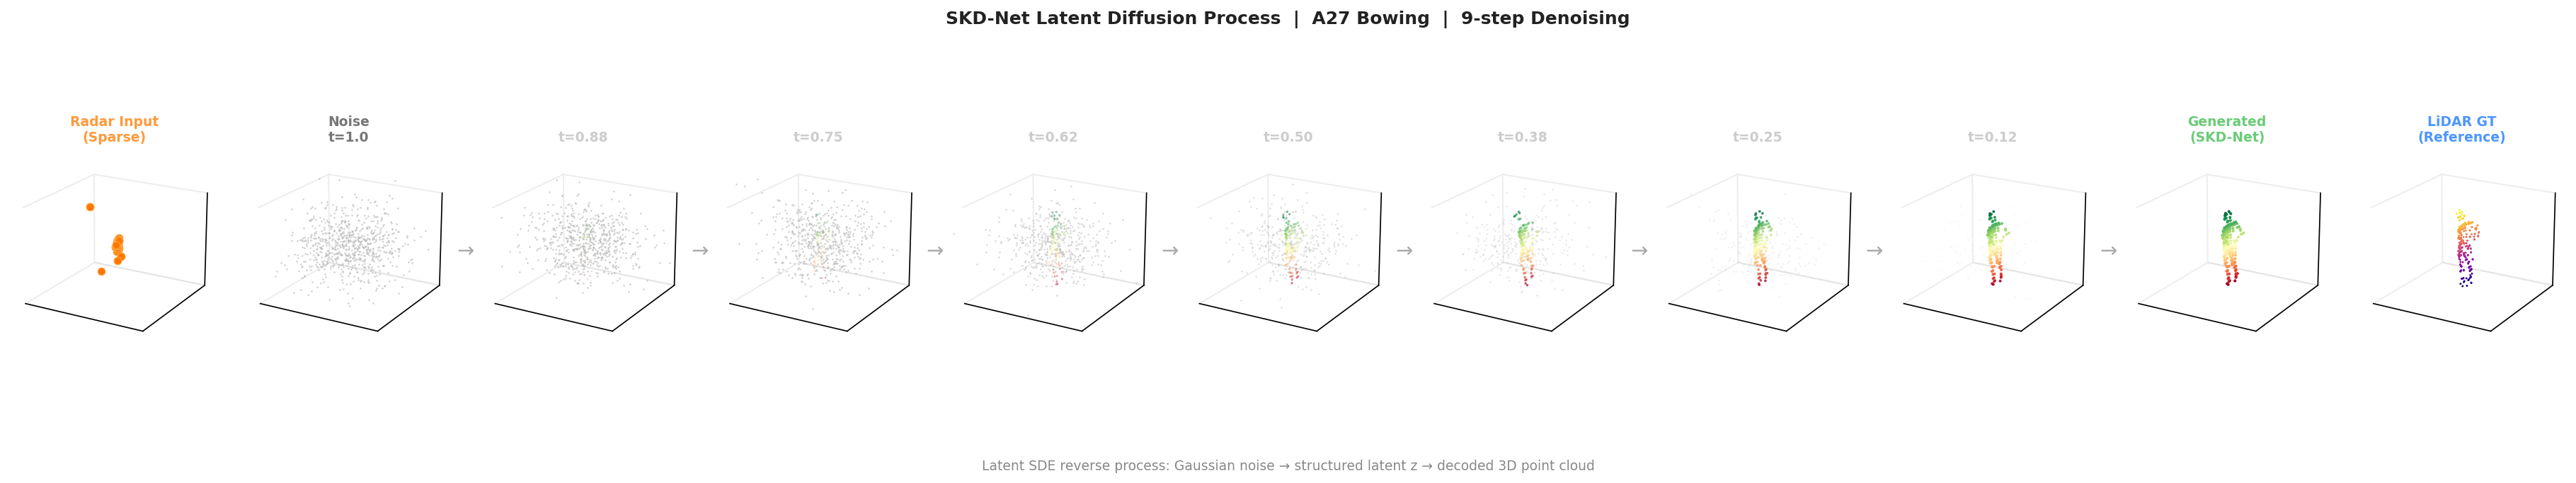
\includegraphics[width=\linewidth]{assets/diffusion_process.png}
  \caption{
    \textbf{Latent SDE reverse process (A27 Bowing).}
    Noise at $t\!=\!1.0$ (left) progressively condenses to a structured human
    point cloud at $t\!=\!0$ (right).
    An auxiliary point-cloud-space noise overlay, proportional to $t$ and in the
    same color as the body, illustrates the ``same-color condensation'' effect
    without artificially separating noise from signal.
  }
  \label{fig:diffusion_process}
\end{figure}

\section{Per-Action Denoising Grid}
\label{app:grid}

Figure~\ref{fig:diffusion_grid} shows the denoising process for all 8 training
actions on representative frames
(S01: A03/fr29, A12/fr8, A13/fr73, A19/fr59, A22/fr50, A26/fr40, A27/fr51,
A17/fr44), generated by \texttt{vis\_diffusion\_grid.py}.

\begin{figure}[h]
  \centering
  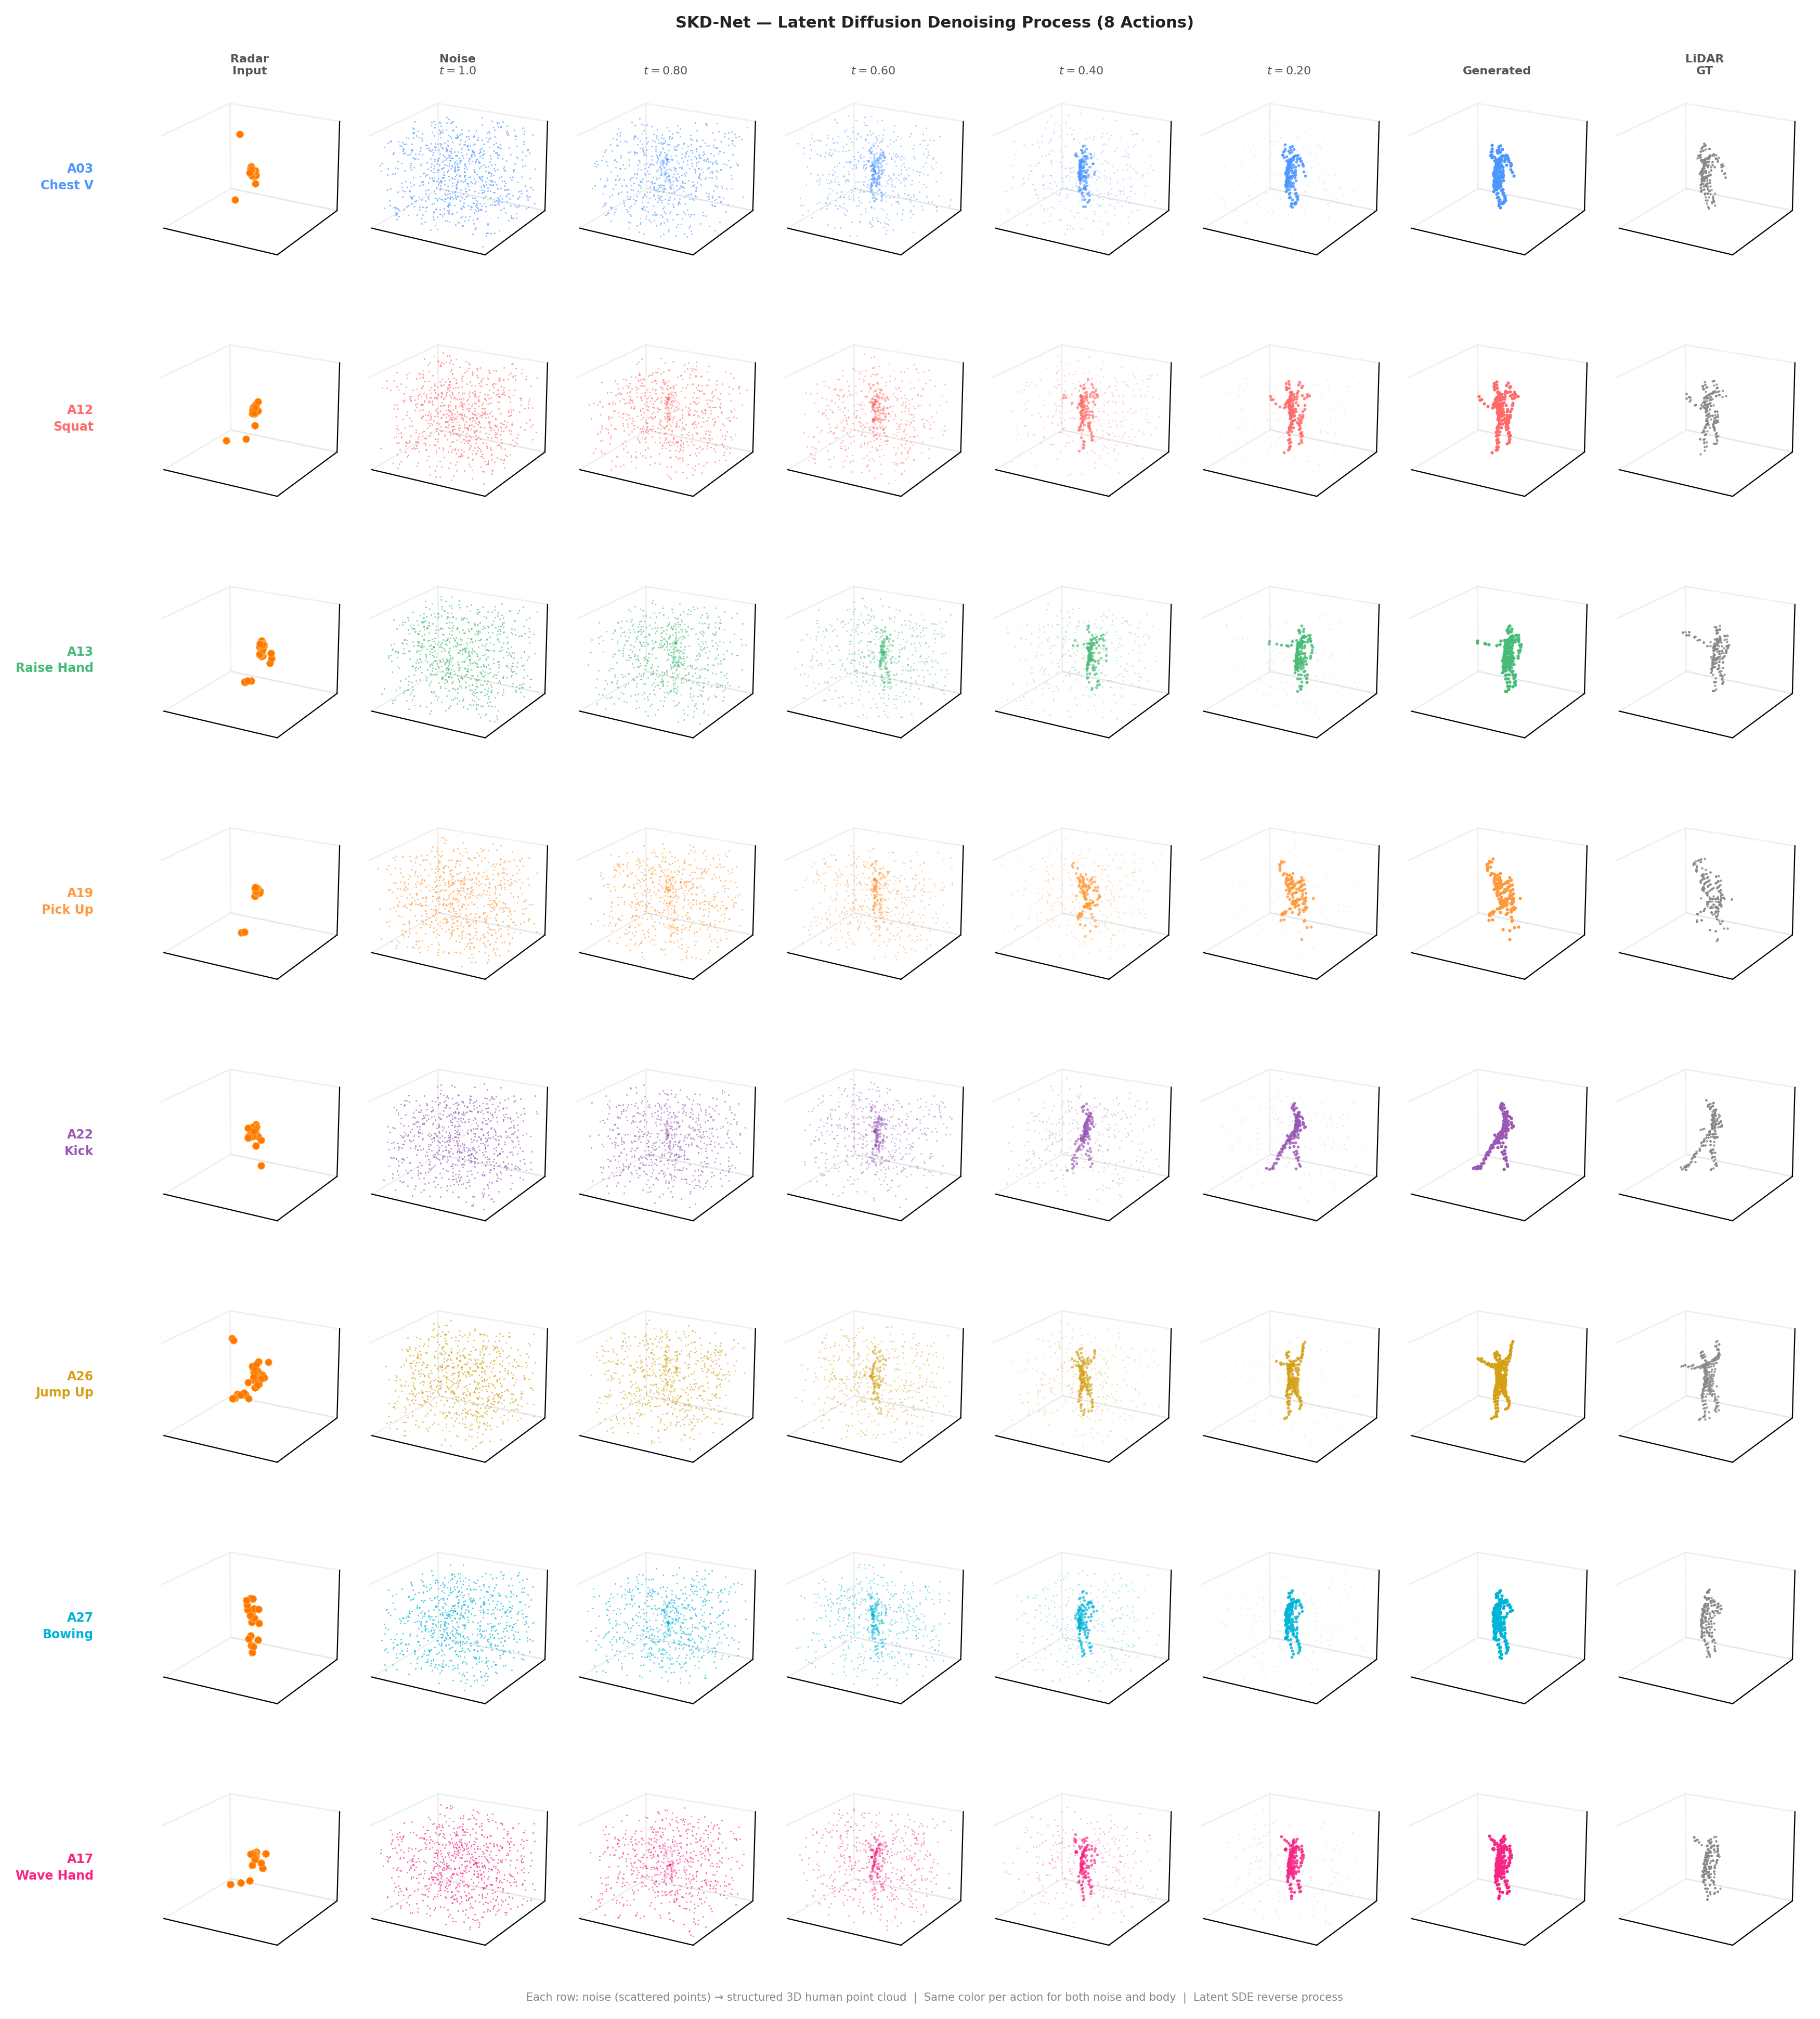
\includegraphics[width=\linewidth]{assets/diffusion_grid.png}
  \caption{
    \textbf{Per-action denoising grid (8 training actions).}
    Each row: one action; columns: noise $\to$ human denoising steps.
    Same-color noise/body convention makes the cloud-condensation effect clear.
  }
  \label{fig:diffusion_grid}
\end{figure}

\section{Additional Qualitative Results}
\label{app:extra_qual}

\todo{Per-subject and per-action qualitative completion grids.}

\section{Reproducibility Details}
\label{app:repro}

\begin{itemize}[leftmargin=1.5em,itemsep=2pt]
  \item \textbf{Dataset:} MM-Fi is publicly available~\cite{yang2023mmfi}.
        OccluRadar-Human will be released upon acceptance.
  \item \textbf{Code \& checkpoints:} Full training/evaluation code and best
        checkpoints will be released at \todo{anonymous URL}.
  \item \textbf{Random seed:} 2023 for all experiments.
  \item \textbf{Hardware:} Single NVIDIA RTX 3090 (24\,GB).\\
        Wall-clock training times:
        Stage~1 (SkelKD, 5000 ep): $\sim$13\,h;\;
        Stage~2 (HierVAE, 2000 ep): $\sim$46\,h;\;
        Stage~3 (LDT, 5000 ep): $\sim$4\,h.
\end{itemize}

\end{document}
